\chapter{Implementazione}

\section{Ambiente di Sviluppo e Gestione delle Dipendenze}

Lo sviluppo della libreria è stato effettuato utilizzando \textit{Python} 3.11, con le seguenti versioni delle principali librerie di raccomandazione:

\begin{itemize}
  \item \textit{Surprise} 1.1.4
  \item \textit{Implicit} 0.7.2
  \item \textit{LightFM} 1.17
\end{itemize}

A causa di incompatibilità tra \textit{Surprise} e le versioni più recenti di \textit{NumPy}, è stato necessario utilizzare la versione 1.24.4 di \textit{NumPy}. Tale scelta non ha comportato problemi di compatibilità con le altre librerie utilizzate.

Per la gestione dei pacchetti e delle dipendenze è stato utilizzato \textit{uv}, un gestore di pacchetti Python di nuova generazione sviluppato da \textit{Astral} (gli stessi creatori di \textit{ruff}). Scritto in \textit{Rust}, \textit{uv} si distingue per le sue elevate prestazioni, risultando fino a 10--100 volte più veloce rispetto a \textit{pip}.

Oltre a offrire un'interfaccia compatibile con \textit{pip}, \textit{uv} integra diverse funzionalità avanzate, tra cui:

\begin{itemize}
  \item creazione e gestione di ambienti virtuali (\texttt{uv venv});
  \item risoluzione e sincronizzazione delle dipendenze con lockfile universali (\texttt{uv pip compile}, \texttt{uv pip sync})
  \item installazione di pacchetti da file standard come \texttt{requirements.txt} e \\ \texttt{pyproject.toml}
  \item supporto per installazioni da repository \textit{Git}, URL e pacchetti locali
\end{itemize}

\section{Implementazione dei modelli}

\subsection{Surprise}

La classe astratta \texttt{SurpriseModel} implementa internamente la logica per la gestione del \textit{dataset} e il salvataggio dei modelli. 

Alcune considerazioni sull'implementazione:

\begin{itemize}
    \item per l'addestramento e la previsione viene utilizzata la struttura dati \\ \texttt{surprise.dataset.Dataset}, creata con la chiamata al metodo statico \\ \texttt{load\_from\_df} utilizzando direttamente dai dati passati tramite le funzioni \texttt{fit} e \texttt{predict}. Il valore del parametro \texttt{rating\_scale} dell'oggetto \\ \texttt{surprise.reader.Reader}, che viene utilizzato per la creazione dell'oggetto \texttt{Dataset}, viene impostato come \texttt{(rating\_column.min, \\ rating\_column.max)}. Se non sono presenti i \textit{rating} nel \textit{trainset}, il valore di default viene impostato a \texttt{(0, 1)}
    \item per il salvataggio, all'interno del metodo \texttt{save} viene utilizzato il metodo \texttt{pickle.dump} per serializzare il modello
    \item il metodo statico \texttt{load} che implementa ogni sottoclasse utilizza invece il metodo \texttt{pickle.load} per deserializzare il file salvato e ricostruire il modello
\end{itemize}

\subsection{Implicit}

La classe astratta \texttt{ImplicitModel} implementa internamente la logica per la gestione del \textit{dataset} e il salvataggio dei modelli. 

Alcune considerazioni sull'implementazione:

\begin{itemize}
    \item per l'addestramento e la previsione i dati vengono convertiti da \textit{DataFrame} a \textit{csr\_matrix}. Per prima cosa si crea e si salva una versione \textit{encoded}, tramite l'oggetto \texttt{sklearn.preprocessing.LabelEncoder} dei vari id. Viene creata una matrice in formato \textit{COO} utilizzando la funzione \texttt{sparse.coo\_matrix} della libreria \textit{Scipy}. In questo passaggio, se nel \textit{trainset} non è presente la terza colonna contenente i pesi dell'interazione, viene aggiunta una colonna \textit{placeholder} tutta con valore 1. Infine la matrice viene convertita in formato \textit{CSR} tramite la funzione \texttt{coo\_matrix.tocsr()} 
    \item per il salvataggio, all'interno del metodo \texttt{save} viene utilizzato il metodo \texttt{save} già presente nei modelli di \textit{Implicit} che salva il modello usando il formato \textit{.npz} di \textit{NumPy}
    \item il metodo statico \texttt{load} che implementa ogni sottoclasse utilizza invece il metodo \texttt{load} che ogni modello \textit{Implicit} già implementa
\end{itemize}

\subsection{LightFM}

La classe \texttt{LightFM} implementa internamente la logica per la gestione del \textit{dataset} e il salvataggio dei modelli. 

Alcune considerazioni sull'implementazione:

\begin{itemize}
    \item per l'addestramento e la previsione i dati vengono convertiti da \textit{DataFrame} a \textit{coo\_matrix}. Per prima cosa si crea e si salva una versione \textit{encoded}, tramite l'oggetto \texttt{sklearn.preprocessing.LabelEncoder} dei vari id. Viene creata una matrice in formato \textit{COO} utilizzando il metodo \texttt{build\_interactions} dell'oggetto \texttt{lightfm.data.Dataset}. In questo passaggio, se nel \textit{trainset} non è presente la terza colonna contenente i pesi dell'interazione, viene aggiunta una colonna \textit{placeholder} tutta con valore 1. 
    \item se sono presenti delle features vengono chiamati i metodi \\ \texttt{build\_item\_features} e \texttt{build\_user\_features} dell'oggetto \\ \texttt{lightfm.data.Dataset} per creare le features degli \textit{item} e degli \textit{user}
    \item per il salvataggio, all'interno del metodo \texttt{save} viene utilizzato il metodo \texttt{pickle.dump} per serializzare il modello
    \item il metodo statico \texttt{load} utilizza invece il metodo \texttt{pickle.load} per deserializzare il file salvato e ricostruire il modello
\end{itemize}

\section{Parametri appresi}

Affinché qualunque istanza di una classe che estenda \texttt{BaseModel} si possa considerare addestrata deve esporre almeno un campo il cui nome termini con "\_". Di seguito vengono definiti quali campi vengono esposti da ciascun \textit{transformer} e ciascun modello. Alcuni \textit{transformers}, data la loro natura \textit{stateless}, non apprendono nulla e, di conseguenza, non espongono nessun nuovo campo.

Per i \textit{transformers}:

\begin{itemize}
    \item \texttt{LabelEncoder}: \texttt{classes\_}, un array che contenente un'etichetta per ciascuna classe
    \item \texttt{Bin}: \texttt{bin\_edges\_} con intervalli dei bin appresi
    \item \texttt{StandardScaler}:
    \begin{itemize}
        \item \texttt{scale\_} : scala relativa per ogni feature dei dati per ottenere media zero e varianza unitaria. Generalmente calcolata come \texttt{np.sqrt(var\_)}. Se la varianza è zero, non si può ottenere varianza unitaria e il fattore di scala è 1. È \texttt{None} se \texttt{with\_std=False}
        \item \texttt{mean\_} : valore medio per ogni feature nel set di addestramento. È \texttt{None} se \texttt{with\_mean=False} e \texttt{with\_std=False}
        \item \texttt{var\_} : varianza per ogni feature nel set di addestramento, usata per calcolare \texttt{scale\_}. È \texttt{None} se \texttt{with\_mean=False} e \texttt{with\_std=False}
        \item \texttt{n\_features\_in\_} : numero di feature viste durante il \texttt{fit}
        \item \texttt{feature\_names\_in\_} : nomi delle feature viste durante il \texttt{fit}, definiti solo se \texttt{X} ha nomi di feature tutti stringa
        \item \texttt{n\_samples\_seen\_} : numero di campioni processati dal modello per ogni feature. Se non ci sono dati mancanti è un intero, altrimenti un array di interi. Se si usano pesi campionari è un float o un array di float che somma i pesi finora visti. Viene azzerato ad ogni nuova chiamata a \texttt{fit}, ma incrementa nelle chiamate a \texttt{partial\_fit}
        \item \texttt{inverse\_transformers\_} : dizionario che contiene le funzioni di trasformazione inversa apprese, usato per applicare trasformazioni inverse specifiche su feature o gruppi di feature
    \end{itemize}
    \item \texttt{Normalizer}:
    \begin{itemize}
        \item \texttt{n\_features\_in\_} : numero di feature viste durante il \texttt{fit}
        \item \texttt{feature\_names\_in\_} : nomi delle feature viste durante il \texttt{fit}, definiti solo se \texttt{X} ha nomi delle feature tutti di tipo stringa
        \item \texttt{transformers\_} : dizionario che contiene le funzioni di trasformazione apprese, usato per applicare trasformazioni specifiche su feature o gruppi di feature
    \end{itemize}
    \item \texttt{OneHotEncode}: 
    \begin{itemize}
        \item \texttt{categories\_list\_} : liste di array contenenti le categorie di ogni feature determinate durante il \texttt{fit}, ordinate come le feature in \texttt{X} e corrispondenti all'output della trasformazione. Include la categoria specificata in \texttt{drop}, se presente
        \item \texttt{drop\_idx\_} : array di dimensione \texttt{(n\_features,)} con l'indice della categoria da scartare per ogni feature. Se non c'è nessuna categoria da scartare, il valore è \texttt{None}. Può essere \texttt{None} anche se tutte le feature sono mantenute. Se sono abilitate categorie infrequenti tramite \texttt{min\_frequency} o \texttt{max\_categories}, e l'indice corrisponde a una categoria infrequente, tutta la categoria infrequente viene scartata
        \item \texttt{infrequent\_categories\_list\_} : array contenente le categorie infrequenti per ogni feature
        \item \texttt{n\_features\_in\_} : numero di feature viste durante il \texttt{fit}
        \item \texttt{feature\_names\_in\_} : nomi delle feature viste durante il \texttt{fit}, se disponibili
        \item \texttt{feature\_name\_combiner} : funzione con \textit{signature} \\ \texttt{def callable(input\_feature, category)} che restituisce una stringa usata per creare i nomi delle feature da restituire con \\ \texttt{get\_feature\_names\_out}
    \end{itemize}
    \item \texttt{MinMaxScaler}:
    \begin{itemize}
        \item \texttt{min\_} : aggiustamento per ogni feature del valore minimo. Equivale a \\ \texttt{min - X.min(axis=0) * scale\_}
        \item \texttt{scale\_} : scala relativa per ogni feature dei dati. Equivale a \\ \texttt{(max - min) / (X.max(axis=0) - X.min(axis=0))}
        \item \texttt{data\_min\_} : minimo osservato per ogni feature nei dati
        \item \texttt{data\_max\_} : massimo osservato per ogni feature nei dati
        \item \texttt{data\_range\_} : intervallo (massimo - minimo) osservato per ogni feature nei dati
        \item \texttt{n\_features\_in\_} : numero di feature viste durante il \texttt{fit}
        \item \texttt{n\_samples\_seen\_} : numero di campioni elaborati dall'estimatore
        \item \texttt{feature\_names\_in\_} : nomi delle feature viste durante il \texttt{fit}, se disponibili
        \item \texttt{transformers\_} : dizionario che contiene le funzioni di trasformazione apprese, usato per applicare trasformazioni specifiche su feature o gruppi di feature
        \item \texttt{inverse\_transformers\_} : dizionario che contiene le funzioni di trasformazione inversa apprese, usato per applicare trasformazioni inverse specifiche su feature o gruppi di feature
    \end{itemize}
    \item \texttt{BinDensity} e \texttt{BinCumulative}:
    \begin{itemize}
        \item \texttt{feature\_values\_} : insieme dei valori presenti nella colonna del feature durante il \textit{fit}
        \item \texttt{excluded\_features\_} : sottoinsieme di valori identificati per essere esclusi (definiti dalla logica di split)
        \item \texttt{grouped\_features\_} : sottoinsieme di valori raggruppati (definiti dalla logica di split)
    \end{itemize}
\end{itemize}

Tutti i modelli apprendono ed espongono come attributi anche \texttt{user\_ids\_} e \texttt{item\_ids\_} e \texttt{train\_user\_item\_pairs\_}, che corrispondono rispettivamente a due liste ordinate degli id di \texttt{user} e \texttt{item} e ad un set di coppie (\textit{user\_id}, \textit{item\_id}) viste durante l'addestramento. Questi valori vengono anche utilizzati dalle funzioni di evaluation implicite~\ref{evaluation_implementation}, quindi i modelli che intendono utilizzare le implementazioni proposte devono esporre questi attributi.

Gli altri attributi sono:

\begin{itemize}
    \item \texttt{ALS}, \texttt{BPR} e \texttt{LMF}:
    \begin{itemize}
        \item \texttt{item\_factors\_} : dizionario contenente, per ogni \textit{item} id, i fattori latenti appresi
        \item \texttt{user\_factors\_} : dizionario contenente, per ogni \textit{user} id, i fattori latenti appresi
    \end{itemize}
    \item \texttt{SVD}, \texttt{SVDpp} e \texttt{NMF}:
    \begin{itemize}
        \item \texttt{pu\_} : dizionario che contiene, per ogni \textit{user} id, i fattori latenti appresi. Ogni valore ha dimensione \textit{num. factors}
        \item \texttt{qi\_} : dizionario che contiene, per ogni \textit{item} id, i fattori latenti appresi. Ogni valore ha dimensione \textit{num. factors}
        \item \texttt{yj\_} (solo \texttt{SVDpp}) : dizionario che contiene, per ogni \textit{item} id, i fattori impliciti appresi. Ogni valore ha dimensione \textit{num. factors}. Serve a modellare il comportamento implicito degli \textit{user}
        \item \texttt{bu\_} : dizionario che contiene, per ogni \textit{user} id, il bias di quello \textit{user}
        \item \texttt{bi\_} : dizionario che contiene, per ogni \textit{item} id, il bias di quell'\textit{item}
    \end{itemize}
    \item \texttt{KNNBaseline}: 
    \begin{itemize}
        \item \texttt{xr\_} : dizionario che contiene, per ogni \textit{user}/\textit{item} id, i vettori di riferimento per i \textit{user}/\textit{item} (e.g. vettori dei \textit{user} nel k-NN user-based)
        \item \texttt{yr\_} : dizionario complementare a \texttt{xr\_}
        \item \texttt{n\_xv\_} : numero di elementi nel dataset corrispondenti a \texttt{xr\_} (e.g. numero di \textit{user})
        \item \texttt{n\_y\_} : numero di elementi nel dataset corrispondenti a \texttt{yr\_} (e.g. numero di \textit{item})
        \item \texttt{bx\_} : dizionario che contiene, per ogni \textit{user}/\textit{item} id, il bias dell'elemento corrispondente in \texttt{xr\_} (e.g. bias dei \textit{user})
        \item \texttt{by\_} : dizionario complementare a \texttt{bx\_}
        \item \texttt{k\_} : numero di vicini usati nel \textit{KNN}
    \end{itemize}

    \item \texttt{SlopeOne}:
    \begin{itemize}
        \item \texttt{freq\_} : dizionario delle frequenze di co-valutazione tra coppie di \textit{item}. \texttt{freq\_[i][j]} indica il numero di \textit{user} che hanno valutato sia l'\textit{item} \texttt{i} che l'\textit{item} \texttt{j}.
        \item \texttt{dev\_} : dizionario delle differenze medie (deviazioni) tra coppie di \textit{item}. \texttt{dev\_[i][j]} indica la differenza media dei \textit{rating} tra l'\textit{item} \texttt{i} e l'\textit{item} \texttt{j}, calcolata sui soli \textit{user} che hanno valutato entrambi

    \end{itemize}
    \item \texttt{CoCluster}:
    \begin{itemize}
        \item \texttt{avg\_cltr\_i\_} : media dei cluster per \textit{item}
        \item \texttt{avg\_cltr\_u\_} : media dei cluster per \textit{user}
        \item \texttt{avg\_cocltr\_} : media dei \textit{co-cluster}
        \item \texttt{bi\_} : dizionario che contiene, per ogni \textit{item} id, il bias di quell'\textit{item}
        \item \texttt{bu\_} : dizionario che contiene, per ogni \textit{user} id, il bias di quello \textit{user}
        \item \texttt{bsl\_options\_} : opzioni per il calcolo delle baseline
        \item \texttt{cltr\_i\_} : cluster degli \textit{item}
        \item \texttt{cltr\_u\_} : cluster degli \textit{user}
        \item \texttt{item\_mean\_} : dizionario che contiene, per ogni \textit{item} id, la media delle valutazioni di quell'\textit{item}
        \item \texttt{n\_cltr\_i\_} : numero di cluster \textit{item}
        \item \texttt{n\_cltr\_u\_} : numero di cluster \textit{user}
        \item \texttt{n\_epochs\_} : numero di epoche di addestramento
        \item \texttt{user\_mean\_} : dizionario che contiene, per ogni \textit{user} id, la media delle valutazioni di quello \textit{user}
    \end{itemize}
    \item \texttt{LightFM}:
    \begin{itemize}
        \item \texttt{user\_biases\_} : dizionario che contiene, per ogni \textit{user} id, il bias di quello \textit{user}
        \item \texttt{user\_embeddings\_} : dizionario che contiene, per ogni \textit{user} id, la rappresentazione latente di quello \textit{user}. Ogni valore ha dimensione \textit{num. components}
        \item \texttt{item\_biases\_} : dizionario che contiene, per ogni \textit{item} id, il bias di quell'\textit{item}
        \item \texttt{item\_embeddings\_} : dizionario che contiene, per ogni \textit{item} id, la rappresentazione latente di quell'\textit{item}. Ogni valore ha dimensione \textit{num. components}
    \end{itemize}


\begin{lstlisting}[caption=Esempio di utilizzo dei parametri appresi]
light_fm = LightFM(no_components=30)
# light_fm.user_embeddings_ 
# raises NotFittedError because models is not fitted yet
light_fm.fit(train, epochs=20)
print(light_fm.user_embeddings_) # shows a matrix of shape (num_users, 30)
\end{lstlisting}

\end{itemize}

\section{Calcolo della similarità item-item e user-user}

Per ciascun modello che estende l'interfaccia \texttt{SimilarityModel} viene specificato il tipo di similarità utilizzata e come viene calcolata.

\begin{itemize}
    \item i modelli \texttt{SVD}, \texttt{SVDpp} e \texttt{NMF} utilizzano la similarità coseno, calcolata tramite la funzione \texttt{cosine\_similarity} di \textit{Scikit-learn}. La matrice di similarità viene calcolata utilizzando \texttt{pu\_} degli \textit{user} o \texttt{qi\_} degli \textit{item} appresi dal modello.
    
    Per \texttt{SVDpp} viene utilizzata anche la rappresentazione implicita degli \textit{item} \texttt{yj\_} per calcolare la rappresentazione dell'\textit{user}:

    \[\vec{p}_u^{\text{ SVD++}} = \vec{p}_u + \frac{1}{|N(u)|} \sum_{j \in N(u)} \vec{y}_j\]

    dove $N(u)$ è l'insieme degli \textit{item} valutati dall'utente

    \item \texttt{KNNBaseline} utilizza la similarità specificata nel parametro \texttt{sim\_options} che può essere similarità coseno, \textit{Pearson} con o senza baseline e \textit{MSD}. Il calcolo viene applicato sui vettori di \texttt{xr\_} e \texttt{yr\_} appresi dal modello. La similarità coseno viene calcolata tramite la funzione \texttt{cosine\_similarity} di \textit{Scikit-learn}, mentre la similarità \textit{Pearson} e \textit{MSD} vengono calcolate tramite le funzioni \texttt{surprise.similarities.pearson} o \\ \texttt{surprise.similarities.pearson\_baseline} e \\ \texttt{surprise.similarities.msd} della libreria \textit{Surprise}
    \item \texttt{LightFM} utilizza la similarità coseno tra le rappresentazioni latenti degli \textit{item} e degli \textit{user} presenti in \texttt{item\_embeddings\_} e \texttt{user\_embeddings\_}. Il calcolo viene effettuato tramite la funzione \texttt{cosine\_similarity} di \textit{Scikit-learn}
    \item \texttt{ALS}, \texttt{BPR} e \texttt{LMF} implementano la similarità tra \textit{item} e \textit{user} utilizzando i metodi \texttt{similar\_user} e \texttt{similar\_item} delle classi base della libreria \textit{Implicit} che internamente utilizzano similarità coseno o \textit{dot product}
\end{itemize}

\section{Scelta dei grafici per la Data Visualization}

Per i grafici generati dalle funzioni presenti nel modulo di \texttt{visualization} si è deciso di utilizzare la libreria \textit{Seaborn}, in quanto offre uno stile grafico gradevole di default, un'integrazione diretta con i \textit{DataFrame} e la possibilità di creare grafici complessi e statisticamente informativi con poche righe di codice.

Un esempio di quello che si può ottenere analizzando \textit{dataset} e features:

\begin{figure}[H]
    \centering

    \begin{subfigure}[b]{0.60\textwidth}
        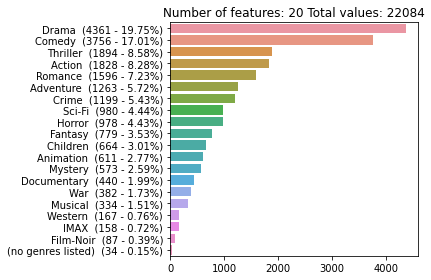
\includegraphics[width=\textwidth]{figures/visualization/output.png}
    \end{subfigure}
    \hfill
    \begin{subfigure}[b]{0.49\textwidth}
        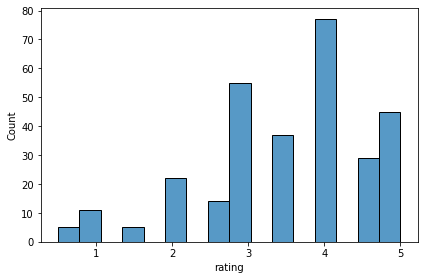
\includegraphics[width=\textwidth]{figures/visualization/output2.png}
    \end{subfigure}
    \hfill
    \begin{subfigure}[b]{0.49\textwidth}
        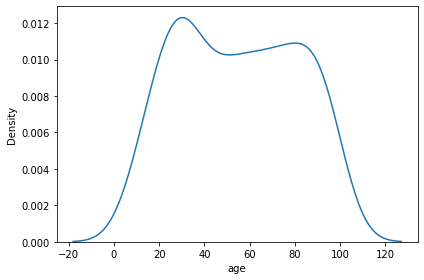
\includegraphics[width=\textwidth]{figures/visualization/output3.png}
    \end{subfigure}

    \caption{Visualizzazione esplorativa dei dati. In alto: distribuzione dei generi cinematografici presenti nel dataset, originariamente uniti in gruppi contenti più generi e uniti dal carattere "|". In basso a sinistra: istogramma delle valutazioni assegnate dagli utenti. In basso a destra: distribuzione delle età degli utenti
}
\end{figure}

\section{Model Selection}

la funzione \texttt{train\_test\_split\_with\_coverage} riceve in ingresso un \textit{DataFrame} o un \textit{NumPy array} contenente le interazioni tra \textit{user} e \textit{item}, e una percentuale (o numero assoluto) che definisce la dimensione del \textit{testset}. L'obiettivo è selezionare casualmente una porzione di interazioni da rimuovere dal \textit{dataset} iniziale, ma solo se la loro rimozione non comporta la perdita completa di informazioni su alcun \textit{user} o \textit{item} nel \textit{trainset}.

L'algoritmo procede nel modo seguente:
\begin{enumerate}
    \item conta per ciascun \textit{user} e ciascun \textit{item} il numero di interazioni
    \item mescola il \textit{dataset} in modo riproducibile (tramite \texttt{random\_state})
    \item itera sul \textit{dataset} cercando di rimuovere righe che non siano le uniche a coinvolgere uno specifico \textit{user} o \textit{item}
    \item appena raggiunta la dimensione desiderata del \textit{testset}, il processo si arresta
    \item in caso non fosse possibile possibile generare un \textit{testset} della dimensione specificata viene sollevata un'eccezione
\end{enumerate}

Questo approccio garantisce che il \textit{trainset} contenga almeno un'interazione per ogni \textit{user} e ogni \textit{item}, evitando problemi di id mai visti durante la predizione.

La funzione \texttt{random\_train\_test\_split} è ispirata alla omonima funzione della libreria \textit{Scikit-learn}, ma i tipo di dati in input e in output è un \textit{DataFrame}.

\section{Evaluation}~\label{evaluation_implementation}

Le funzioni all'interno del modulo di \textit{evaluation} sono state pensate per essere utilizzate all'interno dell'oggetto \texttt{GridSearchCV} di \textit{Scikit-learn}, che permette di effettuare la ricerca dei migliori iperparametri per un modello tramite \textit{cross-validation}.

L'oggetto riceve come parametro \texttt{scoring} una funzione che calcola la metrica di valutazione desiderata. Per i modelli espliciti, le metriche di valutazione \textit{RMSE} e \textit{MAE} sono già presenti all'interno di \textit{Scikit-learn} e non necessitano di adattamenti. 

Tuttavia, per i modelli impliciti, è necessario definire una funzione di valutazione personalizzata che calcoli la metrica desiderata, dato che i modelli non restituiscono direttamente i valori previsti, ma piuttosto degli \textit{score}. Tutte le metriche sono calcolate considerando il \textit{ranking} costruito utilizzando gli \textit{score} di tutti i possibili \textit{item} per tutti i possibili \textit{user}.

Le funzioni di scoring passate al parametro \texttt{scoring} di \textit{Scikit-learn} ricevono in ingresso il modello, \texttt{X}, che corrisponde al \textit{DataFrame} o \textit{NumPy array} di \textit{testset}, e \texttt{y}, non utilizzato ma specificato per compatibilità con la libreria. Il problema è che i modelli hanno bisogno di tutti gli id di \textit{user} e \textit{item} in modo da poter calcolare lo score per tutte le possibili coppie (\textit{user\_id}, \textit{item\_id}); inoltre, alcune di esse erano già presenti nel \textit{trainset} e non devono essere considerate nuovamente. Queste informazioni sono contenute negli attributi \texttt{user\_ids\_}, \texttt{item\_ids\_} e \texttt{train\_user\_item\_pairs\_} che vengono apprese dal modello durante la fase di addestramento.


\begin{figure}[H]
    \centering
    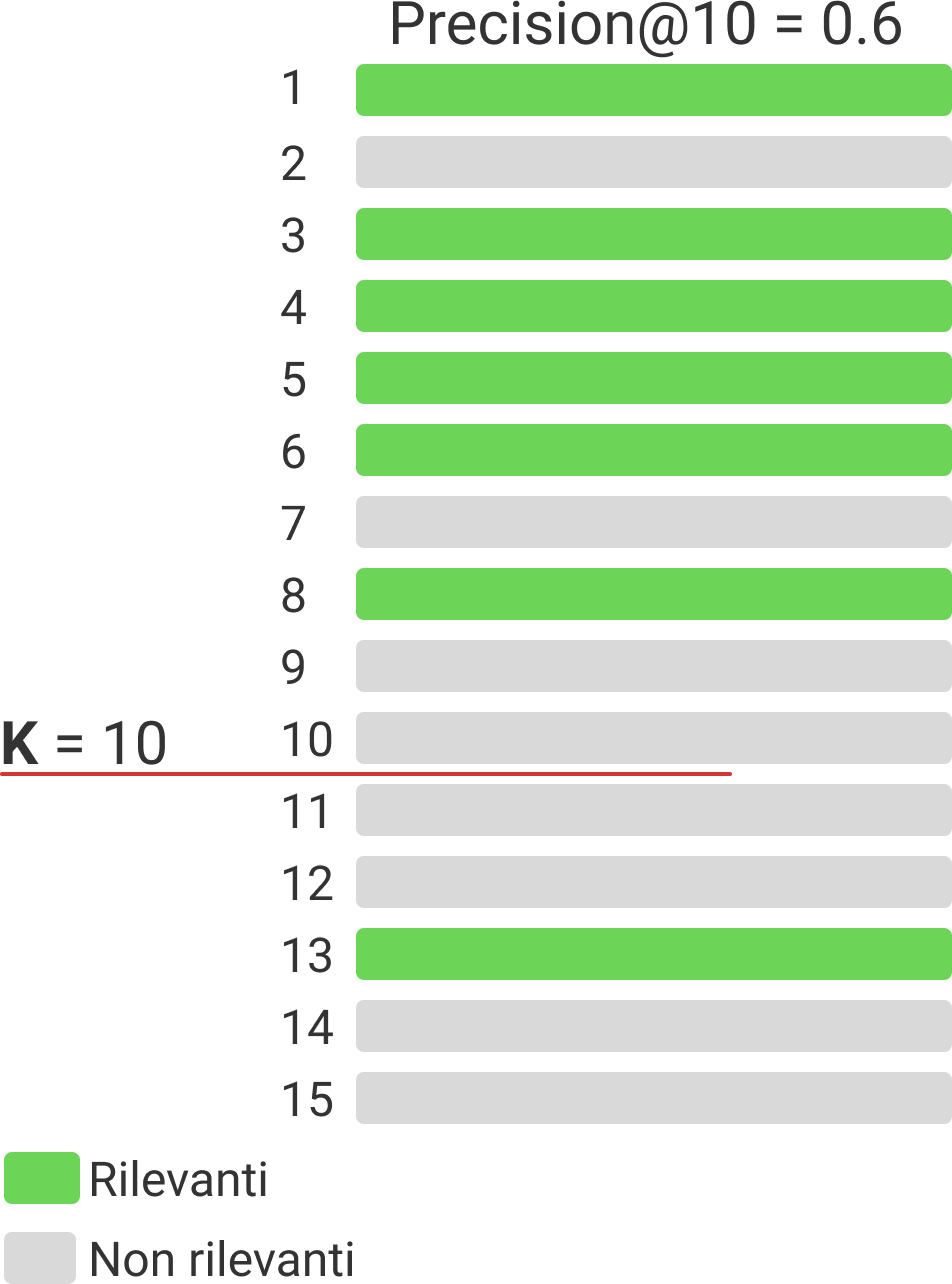
\includegraphics[scale=0.7]{figures/algorithms/precision_@_k.png}
    \caption{L'immagine mostra un esempio di $Precision@10 = 0{.}6$, dove 6 delle 10 raccomandazioni principali risultano \textit{rilevanti} (in verde) e 4 \textit{non rilevanti} (in grigio). La linea rossa evidenzia il cutoff a $K = 10$.}
\end{figure}

Per questo motivo ogni funzione di evaluation all'interno del modulo è stata implementata in due versioni:

\begin{itemize}
    \item funzione normale, con la signature specificata sopra in cui viene chiamata semplicemente la \texttt{predict} del modello
    \item una sua versione \textit{Factory}: questa versione riceve in ingresso una funzione \textit{higher order} \texttt{predict\_fn} e le \textit{keyword args} (\texttt{**kwargs}) di \textit{Python}. \texttt{predict\_fn} verrà chiamata all'interno di una nuova funzione costruita dalla \textit{factory} che avrà la \textit{signature} compatibile con i requisiti di \textit{Scikit-learn}. I \textit{keyword args} verranno passati a \texttt{predict\_fn}. Questo serve per poter dare la possibilità di creare funzioni di metriche custom, per esempio dare la possibilità di poter passare features o parametri aggiuntivi per il metodo \texttt{predict}, come nel caso della classe di \texttt{LightFM} che può ricevere le features di \textit{user} e \textit{item}
    \begin{lstlisting}[caption=Implementazione in pseudo codice di una \textit{factory} per una metrica generica ]
        def metric_factory(predict_fn, **kwargs):
            def metric(model, testset, y=None):
                predictions = predict_fn(model, X, **kwargs)
                # metric computation
                result = ...
                return result
            return metric
    \end{lstlisting}
\end{itemize}